% Copyright 2004 by Till Tantau <tantau@users.sourceforge.net>.
%
% In principle, this file can be redistributed and/or modified under
% the terms of the GNU Public License, version 2.
%
% However, this file is supposed to be a template to be modified
% for your own needs. For this reason, if you use this file as a
% template and not specifically distribute it as part of a another
% package/program, I grant the extra permission to freely copy and
% modify this file as you see fit and even to delete this copyright
% notice. 

\documentclass{beamer}

% There are many different themes available for Beamer. A comprehensive
% list with examples is given here:
% http://deic.uab.es/~iblanes/beamer_gallery/index_by_theme.html
% You can uncomment the themes below if you would like to use a different
% one:
%\usetheme{AnnArbor}
%\usetheme{Antibes}
%\usetheme{Bergen}
%\usetheme{Berkeley}
%\usetheme{Berlin}
%\usetheme{Boadilla}
%\usetheme{boxes}
%\usetheme{CambridgeUS}
%\usetheme{Copenhagen}
%\usetheme{Darmstadt}
%\usetheme{default}
%\usetheme{Frankfurt}
%\usetheme{Goettingen}
%\usetheme{Hannover}
%\usetheme{Ilmenau}
%\usetheme{JuanLesPins}
%\usetheme{Luebeck}
\usetheme{Madrid}
%\usetheme{Malmoe}
%\usetheme{Marburg}
%\usetheme{Montpellier}
%\usetheme{PaloAlto}
%\usetheme{Pittsburgh}
%\usetheme{Rochester}
%\usetheme{Singapore}
%\usetheme{Szeged}
%\usetheme{Warsaw}


% Customize Warsaw color 
\setbeamercolor*{palette primary}{use=structure,fg=white,bg=red!50!black}
\setbeamercolor*{palette secondary}{use=structure,fg=white,bg=red!60!black}
\setbeamercolor*{palette tertiary}{use=structure,fg=white,bg=red!70!black}

% Customize Warsaw block title and background colors
\setbeamercolor{block title}{bg=red!50!black,fg=white}


% List your packages here

\usepackage[colorinlistoftodos]{todonotes}


\title[Progress Update]{A Generalized Open Source Platform for Building Energy Management}

% % A subtitle is optional and this may be deleted
% \subtitle{Product Proposal}

\author[B.~Lauer]{Brian~Lauer\\\and
Advisor: Dr. Suruz Miah}
% - Give the names in the same order as the appear in the paper.
% - Use the \inst{?} command only if the authors have different
%   affiliation.

\institute[Bradley University] % (optional, but mostly needed)
{
  Department of Electrical and Computer Engineering\\
  Bradley University\\
  1501 W. Bradley Avenue\\
  Peoria, IL, 61625, USA
}
% - Use the \inst command only if there are several affiliations.
% - Keep it simple, no one is interested in your street address.

\date[August~20,~2020]{Thursday, August~20,~2020}
% - Either use conference name or its abbreviation.
% - Not really informative to the audience, more for people (including
%   yourself) who are reading the slides online

\logo{\hfill\href{http://www.bradley.edu}{
\includegraphics[width=0.75cm]{../figs/logoBU1-Print}}}  % place logo in every page 


\subject{Mobile Robot Localization}
% Section and subsections will appear in the presentation overview
% and table of contents.
\begin{document}
\begin{frame}
  \titlepage
\end{frame}

\begin{frame}{Outline}
  \tableofcontents
  % You might wish to add the option [pausesections]
\end{frame}
\section{Introduction}

\begin{frame}{Introduction}{}
  % applications of mobile robot navigation and problem description
  \begin{figure}
  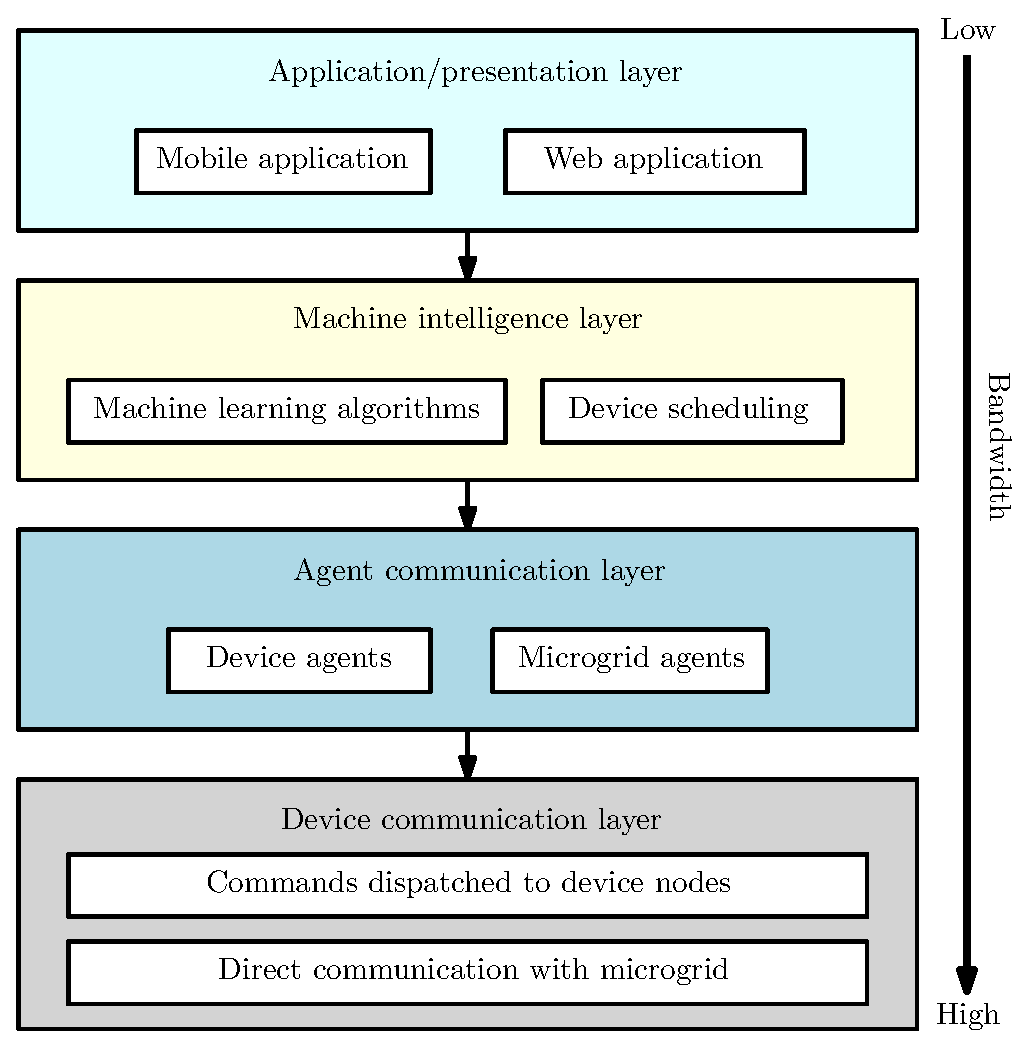
\includegraphics[scale=0.35]{../figs/ipe/BEMS-softwareArchitecture}
  \end{figure}
\end{frame}

\begin{frame}{Introduction}{}
  % applications of mobile robot navigation and problem description
  \begin{figure}
  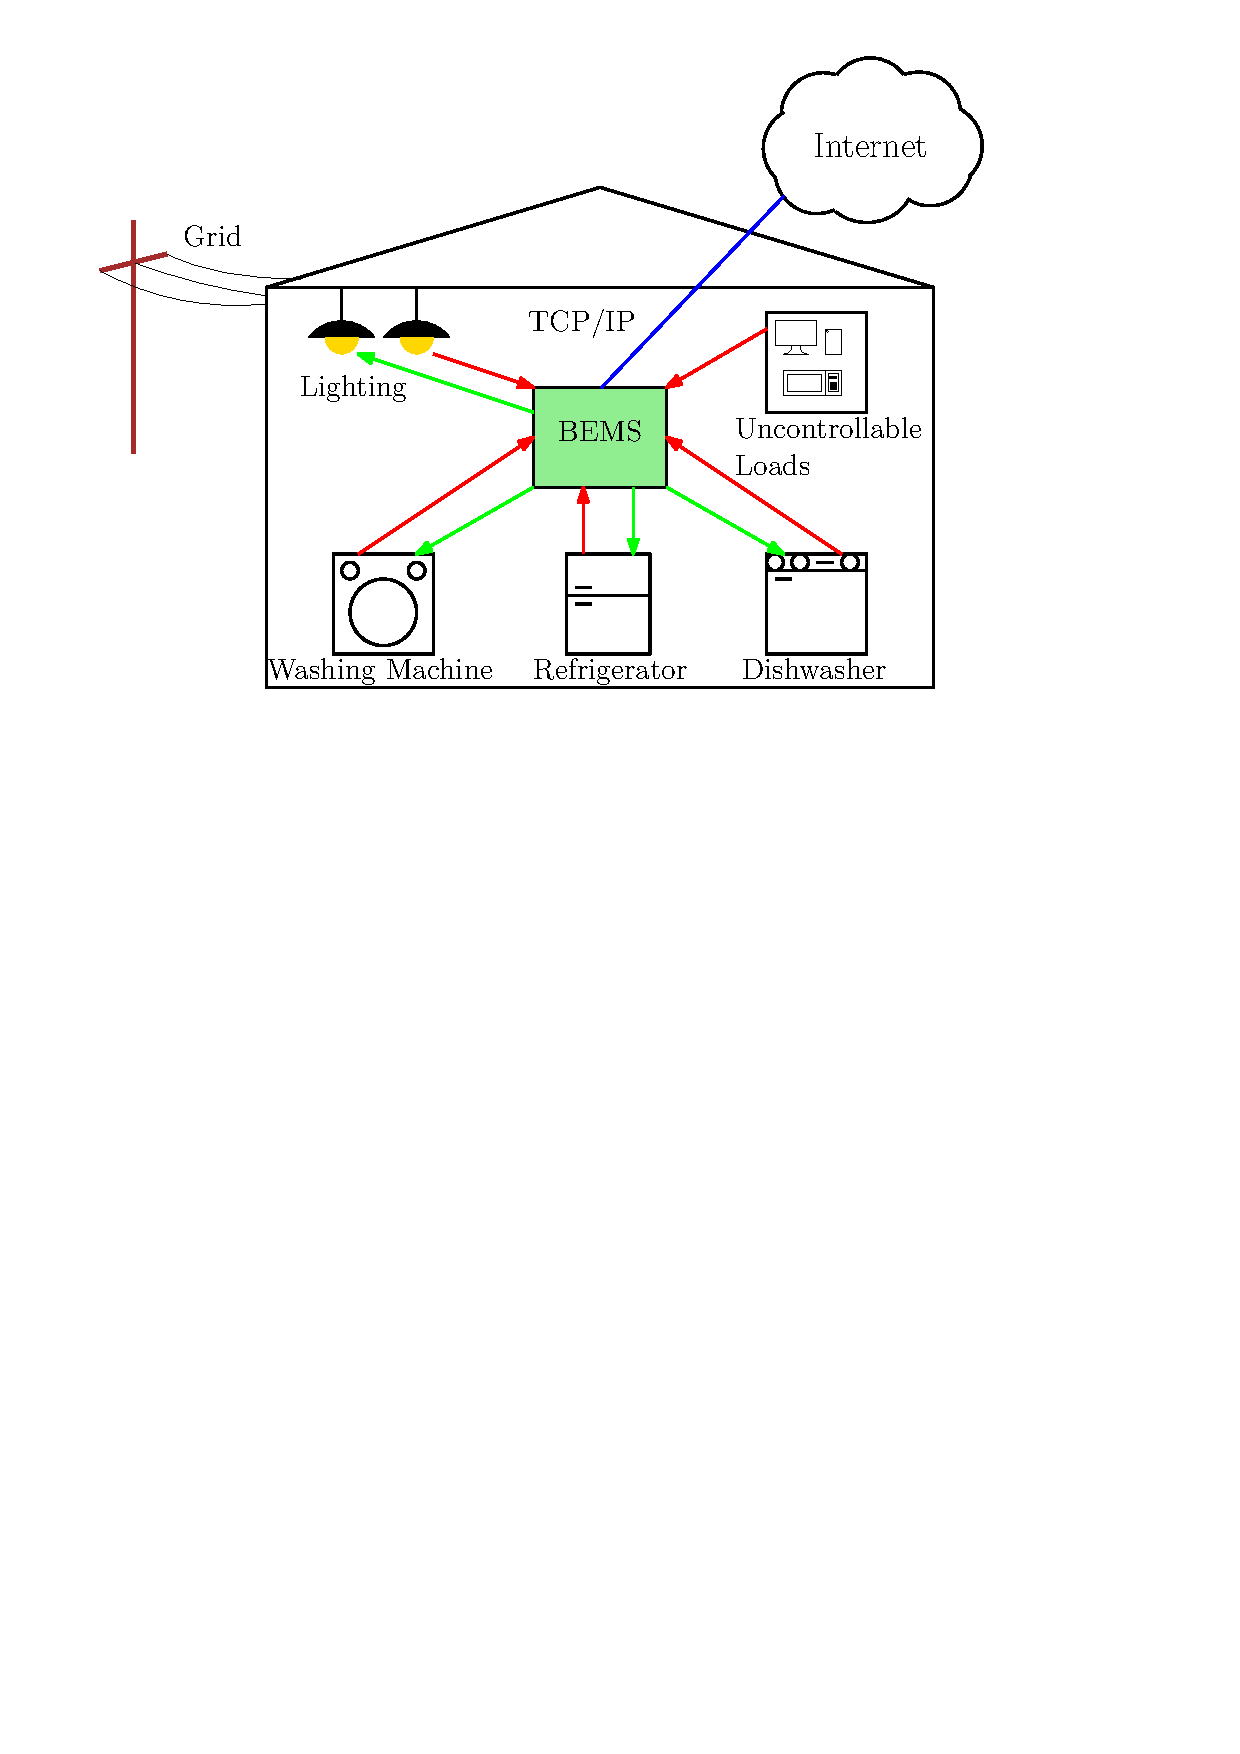
\includegraphics[scale=0.45]{../figs/ipe/bemsdiagram}
  \end{figure}
\end{frame}

\section{Progress}
\begin{frame}{Progress}{}
	\begin{itemize}
		\item Added landing page for '/' and '/home' requests
		\item Added pages for Applications, Notifactions, Settings (only place holder text for now)
		\item Worked on adding a periodic device query feature in the \texttt{ControlAgent}
		\item Attempted to install Git Extensions
	\end{itemize}
\end{frame}

\section{Landing Pages}
\begin{frame}{Landing Pages}{}
\begin{figure}
\centering

\includegraphics[scale=0.25]{../figs/img/landingPage}
\caption{Temporary landing page}
\end{figure}
\end{frame}

\section{Control Agent Work}
\begin{frame}{Control Agent Work}{}
\begin{itemize}
\item Added method \texttt{startPeriodicQueryBehavior} which will start a new thread on method \texttt{periodicQueryBehavior}
\item \texttt{periodicQueryBehavior} will potentially regularly query the device for data and store in the time-series database
\end{itemize}
\end{frame}

\section{Git Extensions}
\begin{frame}{Git Extensions}{}
\begin{figure}
\centering
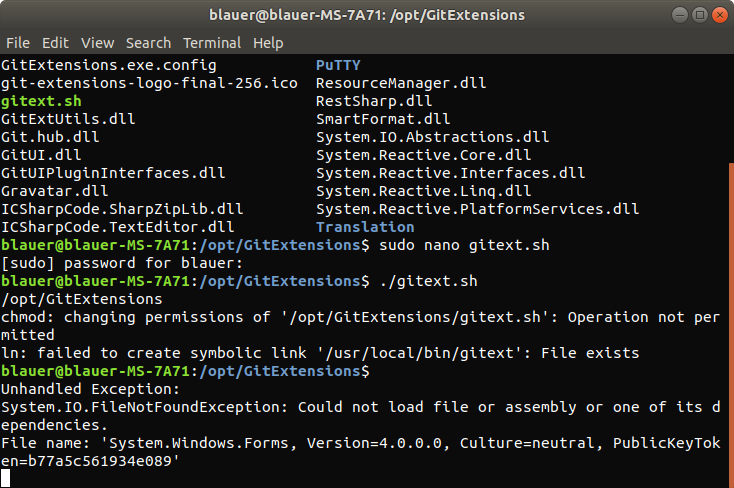
\includegraphics[scale=0.4]{../figs/img/gitExtFileNotFound}
\caption{FileNotFoundException Git Extensions install}
\end{figure}
\end{frame}


\section{Plans}
\begin{frame}{Plans}{}
\begin{itemize}
	\item Determine a time series database (possibly Apache-Cassandra)
	\item Finish up UI and agent work for querying the device for data
	\item Potentially (down the road) integrate a REST API with the software using Flask RESTful
	\item Continue working on installing git extensions
\end{itemize}
\end{frame}

% All of the following is optional and typically not needed. 
\appendix
\section<presentation>*{\appendixname}
\subsection<presentation>*{References}

\begin{frame}[allowframebreaks]
  \frametitle<presentation>{References}
    
  \begin{thebibliography}{10}
    
  \setbeamertemplate{bibliography item}[online]
  
  \bibitem{sems}
  Flask RESTful
  \newblock \url{https://flask-restful.readthedocs.io/en/latest/}
  \end{thebibliography}
\end{frame}

\begin{frame}
\Huge
\center
Any Questions?
\end{frame}
\end{document}


%%% Local Variables:
%%% mode: latex
%%% TeX-master: "../progressPresMain"
%%% End:
